% Supplementary Material S1-S4 (compiled only into arXiv edition via 00_main_arxiv.tex).
% Provenance: Exp 01, Exp 06, Exp 08, Exp 09, and Exp 10.
% One sentence per line (Trigger Rule 13); strictly anonymized.

\FloatBarrier
\clearpage
\setcounter{section}{0}
\renewcommand{\thesection}{S\arabic{section}}
\setcounter{table}{0}
\renewcommand{\thetable}{S\arabic{table}}
\setcounter{figure}{0}
\renewcommand{\thefigure}{S\arabic{figure}}

\section*{Supplementary Material: Extended Tables, Blind Prompt Search, and Validity Boundaries}

\section{Extended Synthetic Tables}
\label{sec:supp-toy}

This section provides the full held-out numerical tables backing the population counterexample and rank-correlation synthetic suites.
Across synthetic suites, predictions are evaluated on $500$ held-out tasks per seed against the analytic data-generating distribution $p(r \mid x)$ across $100$ random seeds, with uncertainty reported as paired $95\%$ percentile bootstrap intervals over $10{,}000$ draws.

\subsection{Population Counterexample and Single-Rating Selection (Experiment 01)}
In the two-point population counterexample with bimodal symmetric task uncertainty versus unimodal spread, all candidate judges $q_\epsilon$ with mixing parameter $\epsilon \in \{0, 0.25, 0.50, 0.75, 0.95\}$ achieve identical normalized mean squared error ($\mathrm{nMSE} = 0.038$) and identical Pearson correlation with the conditional mean.
Table~\ref{tab:supp-exp01} contrasts these scalar metrics against strictly proper distributional scoring rules and reports 256-task single-rating selection recovery.
Cross-entropy (CE) identifies the true distribution in $249/256$ draws (mean held-out CE $1.331$ nats, $95\%$ CI $[1.329, 1.334]$), while Brier score and ranked probability score (RPS) recover it in $245/256$ draws ($1.333$ nats, $95\%$ CI $[1.330, 1.336]$), compared with $1.995$ nats under uniform correlation tie-breaking.

\begin{table}[htb]
\centering
\caption{Experiment~01 population scoring rules across ambiguity perturbations $q_\epsilon$ sharing identical mean rating and identical nMSE ($0.038$), plus sign-reversed control (lower is better).}
\label{tab:supp-exp01}
\small
\setlength{\tabcolsep}{3pt}
\begin{tabular}{@{}lcccc@{}}
\hline
Variant & CE (nats) & Brier & RPS & nMSE \\
\hline
True $q_0$ & $1.328$ & $0.699$ & $0.104$ & $0.038$ \\
$q_{0.25}$ & $1.446$ & $0.733$ & $0.109$ & $0.038$ \\
$q_{0.50}$ & $1.689$ & $0.835$ & $0.125$ & $0.038$ \\
$q_{0.75}$ & $2.164$ & $1.004$ & $0.152$ & $0.038$ \\
$q_{0.95}$ & $3.348$ & $1.188$ & $0.181$ & $0.038$ \\
Reversed $q_{\mathrm{rev}}$ & $4.215$ & $1.113$ & $0.384$ & $0.282$ \\
\hline
\end{tabular}
\end{table}

\subsection{Rank and Mixed Correlation Surrogates (Experiment 06)}
To verify that the synthetic gap is not specific to linear Pearson correlation, Experiment~06 trains the same 78-weight Fourier softmax family on smooth Spearman, smooth Kendall, and half-Pearson half-Spearman surrogates alongside CE and RPS\@.
Figure~\ref{fig:supp-rank} and Table~\ref{tab:supp-exp06} report held-out test RPS excess, test CE excess, and Spearman rank correlation with the true conditional mean across $n \in \{4, 16, 64, 256, 1{,}024, 2{,}048\}$ training tasks (3 ratings per task).
In Scenario~A, CE outperforms Pearson, Spearman, and their equal mixture significantly from $n = 64$ tasks (192 ratings) onward, and outperforms Kendall from $n = 8$ tasks onward; in Scenario~B, CE outperforms every competing objective at every sample size from $n = 4$ onward.
Even at $n=2{,}048$ in Scenario~B where Pearson ($0.973$), Spearman ($0.982$), and Kendall ($0.981$) attain slightly higher rank agreement with the conditional mean than CE ($0.948$), their distribution predictions incur $0.0330$--$0.0951$ test RPS excess and $0.3233$--$0.5957$ nats of CE excess compared with $0.0037$ RPS and $0.0222$ nats for CE\@.

\begin{figure}[t]
\centering
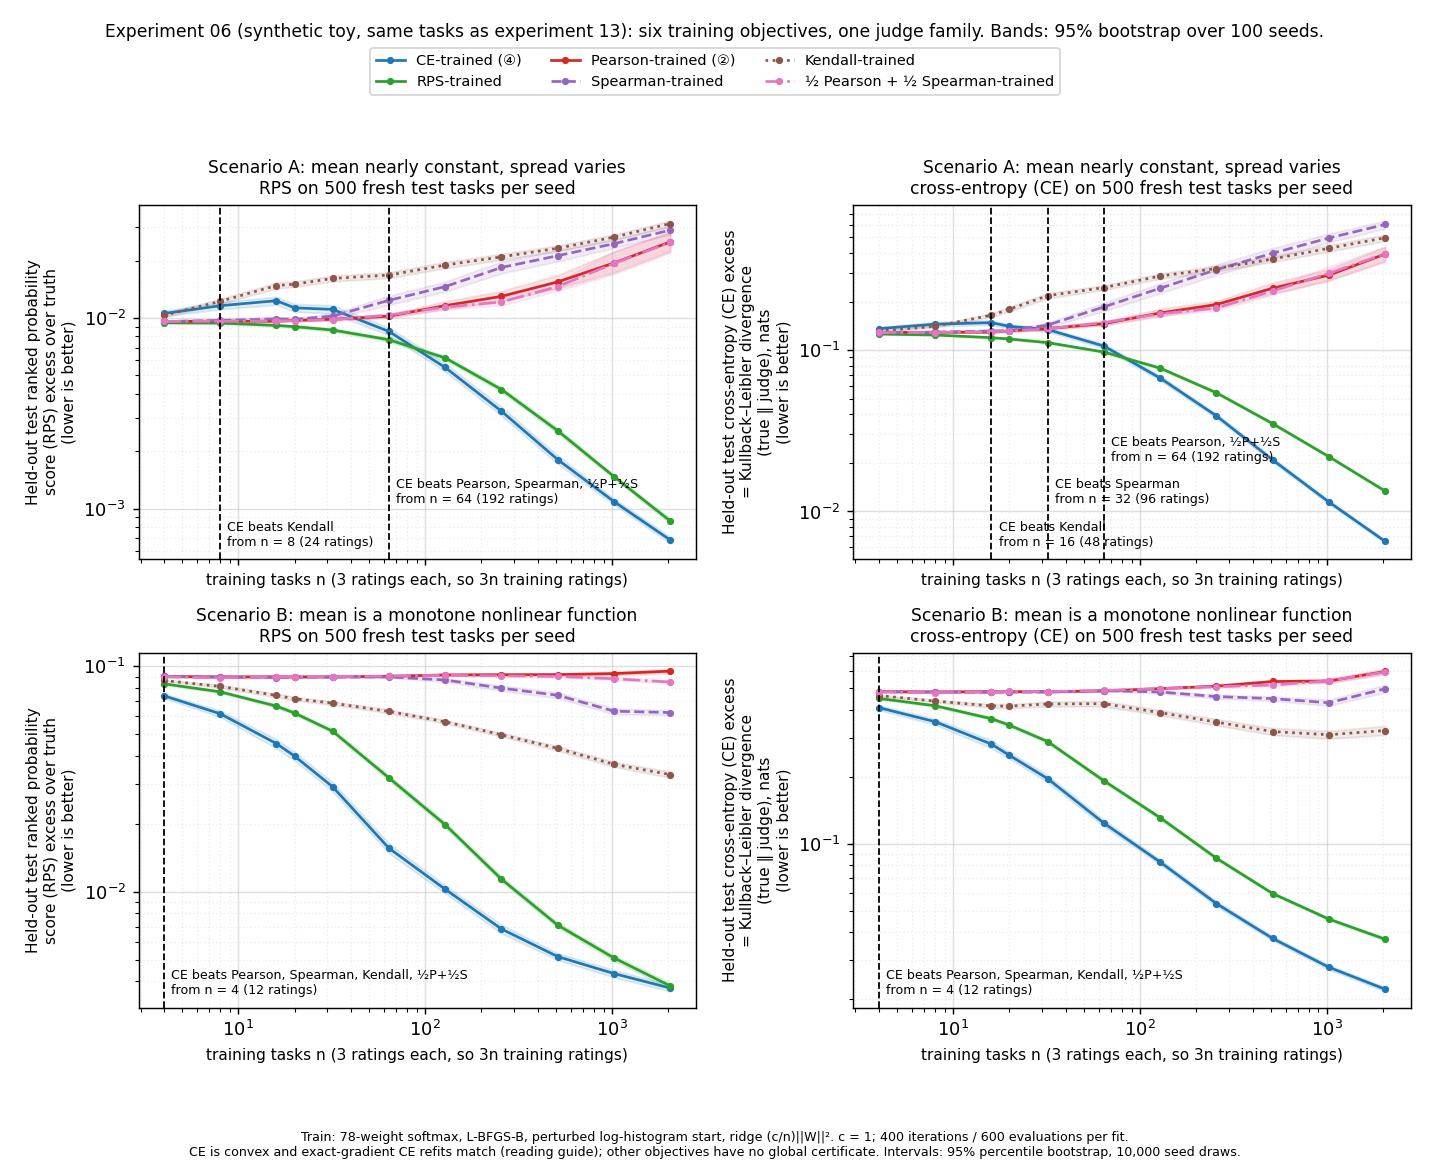
\includegraphics[width=\columnwidth]{figures/fig_rank_objectives_vs_n.png}
\caption{Experiment~06 held-out test RPS excess (left) and CE excess (right) across sample sizes $n$ comparing CE and RPS against Pearson, smooth Spearman, smooth Kendall, and $1/2$ Pearson + $1/2$ Spearman surrogates in Scenarios~A and~B (100 seeds, 500 test tasks per seed, lower is better).}
\label{fig:supp-rank}
\end{figure}

\begin{table*}[t]
\centering
\caption{Experiment~06 held-out test RPS excess over truth across sample sizes $n$ (3 ratings per task; 100 seeds; zero optimal, lower is better) plus $n=2{,}048$ CE excess (nats) and test Spearman rank correlation with the true mean.}
\label{tab:supp-exp06}
\small
\begin{tabular}{@{}lcccccc@{}}
\hline
Scenario / Sample Size & CE-Trained & RPS-Trained & Pearson-Trained & Spearman-Trained & Kendall-Trained & $\tfrac{1}{2}$P + $\tfrac{1}{2}$S \\
\hline
Scenario A, $n=4$ ($12$ ratings) & $0.0106$ & $0.0094$ & $0.0096$ & $0.0096$ & $0.0103$ & $0.0096$ \\
Scenario A, $n=16$ ($48$ ratings) & $0.0123$ & $0.0091$ & $0.0096$ & $0.0099$ & $0.0148$ & $0.0097$ \\
Scenario A, $n=64$ ($192$ ratings) & $0.0085$ & $0.0077$ & $0.0102$ & $0.0124$ & $0.0168$ & $0.0104$ \\
Scenario A, $n=256$ ($768$ ratings) & $0.0032$ & $0.0042$ & $0.0130$ & $0.0184$ & $0.0209$ & $0.0121$ \\
Scenario A, $n=1{,}024$ ($3{,}072$) & $0.0011$ & $0.0015$ & $0.0195$ & $0.0246$ & $0.0266$ & $0.0194$ \\
Scenario A, $n=2{,}048$ RPS Excess & $0.0007$ & $0.0009$ & $0.0251$ & $0.0289$ & $0.0313$ & $0.0249$ \\
Scenario A, $n=2{,}048$ CE Excess & $0.0065$ & $0.0134$ & $0.3937$ & $0.6005$ & $0.4968$ & $0.3954$ \\
\hline
Scenario B, $n=4$ ($12$ ratings) & $0.0740$ & $0.0836$ & $0.0901$ & $0.0901$ & $0.0865$ & $0.0898$ \\
Scenario B, $n=16$ ($48$ ratings) & $0.0454$ & $0.0665$ & $0.0898$ & $0.0891$ & $0.0742$ & $0.0896$ \\
Scenario B, $n=64$ ($192$ ratings) & $0.0156$ & $0.0320$ & $0.0902$ & $0.0896$ & $0.0630$ & $0.0905$ \\
Scenario B, $n=256$ ($768$ ratings) & $0.0068$ & $0.0114$ & $0.0917$ & $0.0800$ & $0.0497$ & $0.0907$ \\
Scenario B, $n=1{,}024$ ($3{,}072$) & $0.0043$ & $0.0051$ & $0.0928$ & $0.0632$ & $0.0367$ & $0.0880$ \\
Scenario B, $n=2{,}048$ RPS Excess & $0.0037$ & $0.0038$ & $0.0951$ & $0.0623$ & $0.0330$ & $0.0851$ \\
Scenario B, $n=2{,}048$ CE Excess & $0.0222$ & $0.0372$ & $0.5957$ & $0.4981$ & $0.3233$ & $0.5919$ \\
Scenario B, $n=2{,}048$ Spearman & $0.948$ & --- & $0.973$ & $0.982$ & $0.981$ & $0.977$ \\
\hline
\end{tabular}
\end{table*}

\subsection{MSE-Trained and Regularized Calibrated-Head Baselines (Experiment 11)}
Experiment~11 evaluates four-fold cross-fitted Stage-2 calibration heads with tuned slope regularization $c_b \in \{0.01, \dots, 10^8\}$ (\texttt{Pearson + tuned head}, \texttt{MSE + tuned head}) and direct 78-weight mean squared error (\texttt{MSE}) training across all four synthetic scenarios~A--D and 100 seeds.
Figure~\ref{fig:supp-exp11} and Table~\ref{tab:supp-exp11} compare held-out test RPS (both relative to truth and raw), CE excess, and paired differences relative to the constant baseline and validation-tuned CE (\textcircled{3}).
Cross-fitting and slope regularization eliminate the small-$n$ calibration spike by $n=32$ ($+0.0006, -0.0004, -0.0004, -0.0002$ vs.\ constant across A--D), and MSE training fixes Pearson's arbitrary affine scaling.
When conditional spread $\kappa(x)$ varies (Scenarios~A and~B), validation-tuned CE beats all 1D score-calibrated and MSE baselines at every sample size ($n \ge 4$); when $\kappa$ is constant (Scenarios~C and~D), low-variance 12-parameter Stage-2 CE calibration heads match or slightly edge out 78-weight CE at $n=2{,}048$ while still depending on proper-loss CE optimization in Stage~2.

\begin{figure}[t]
\centering
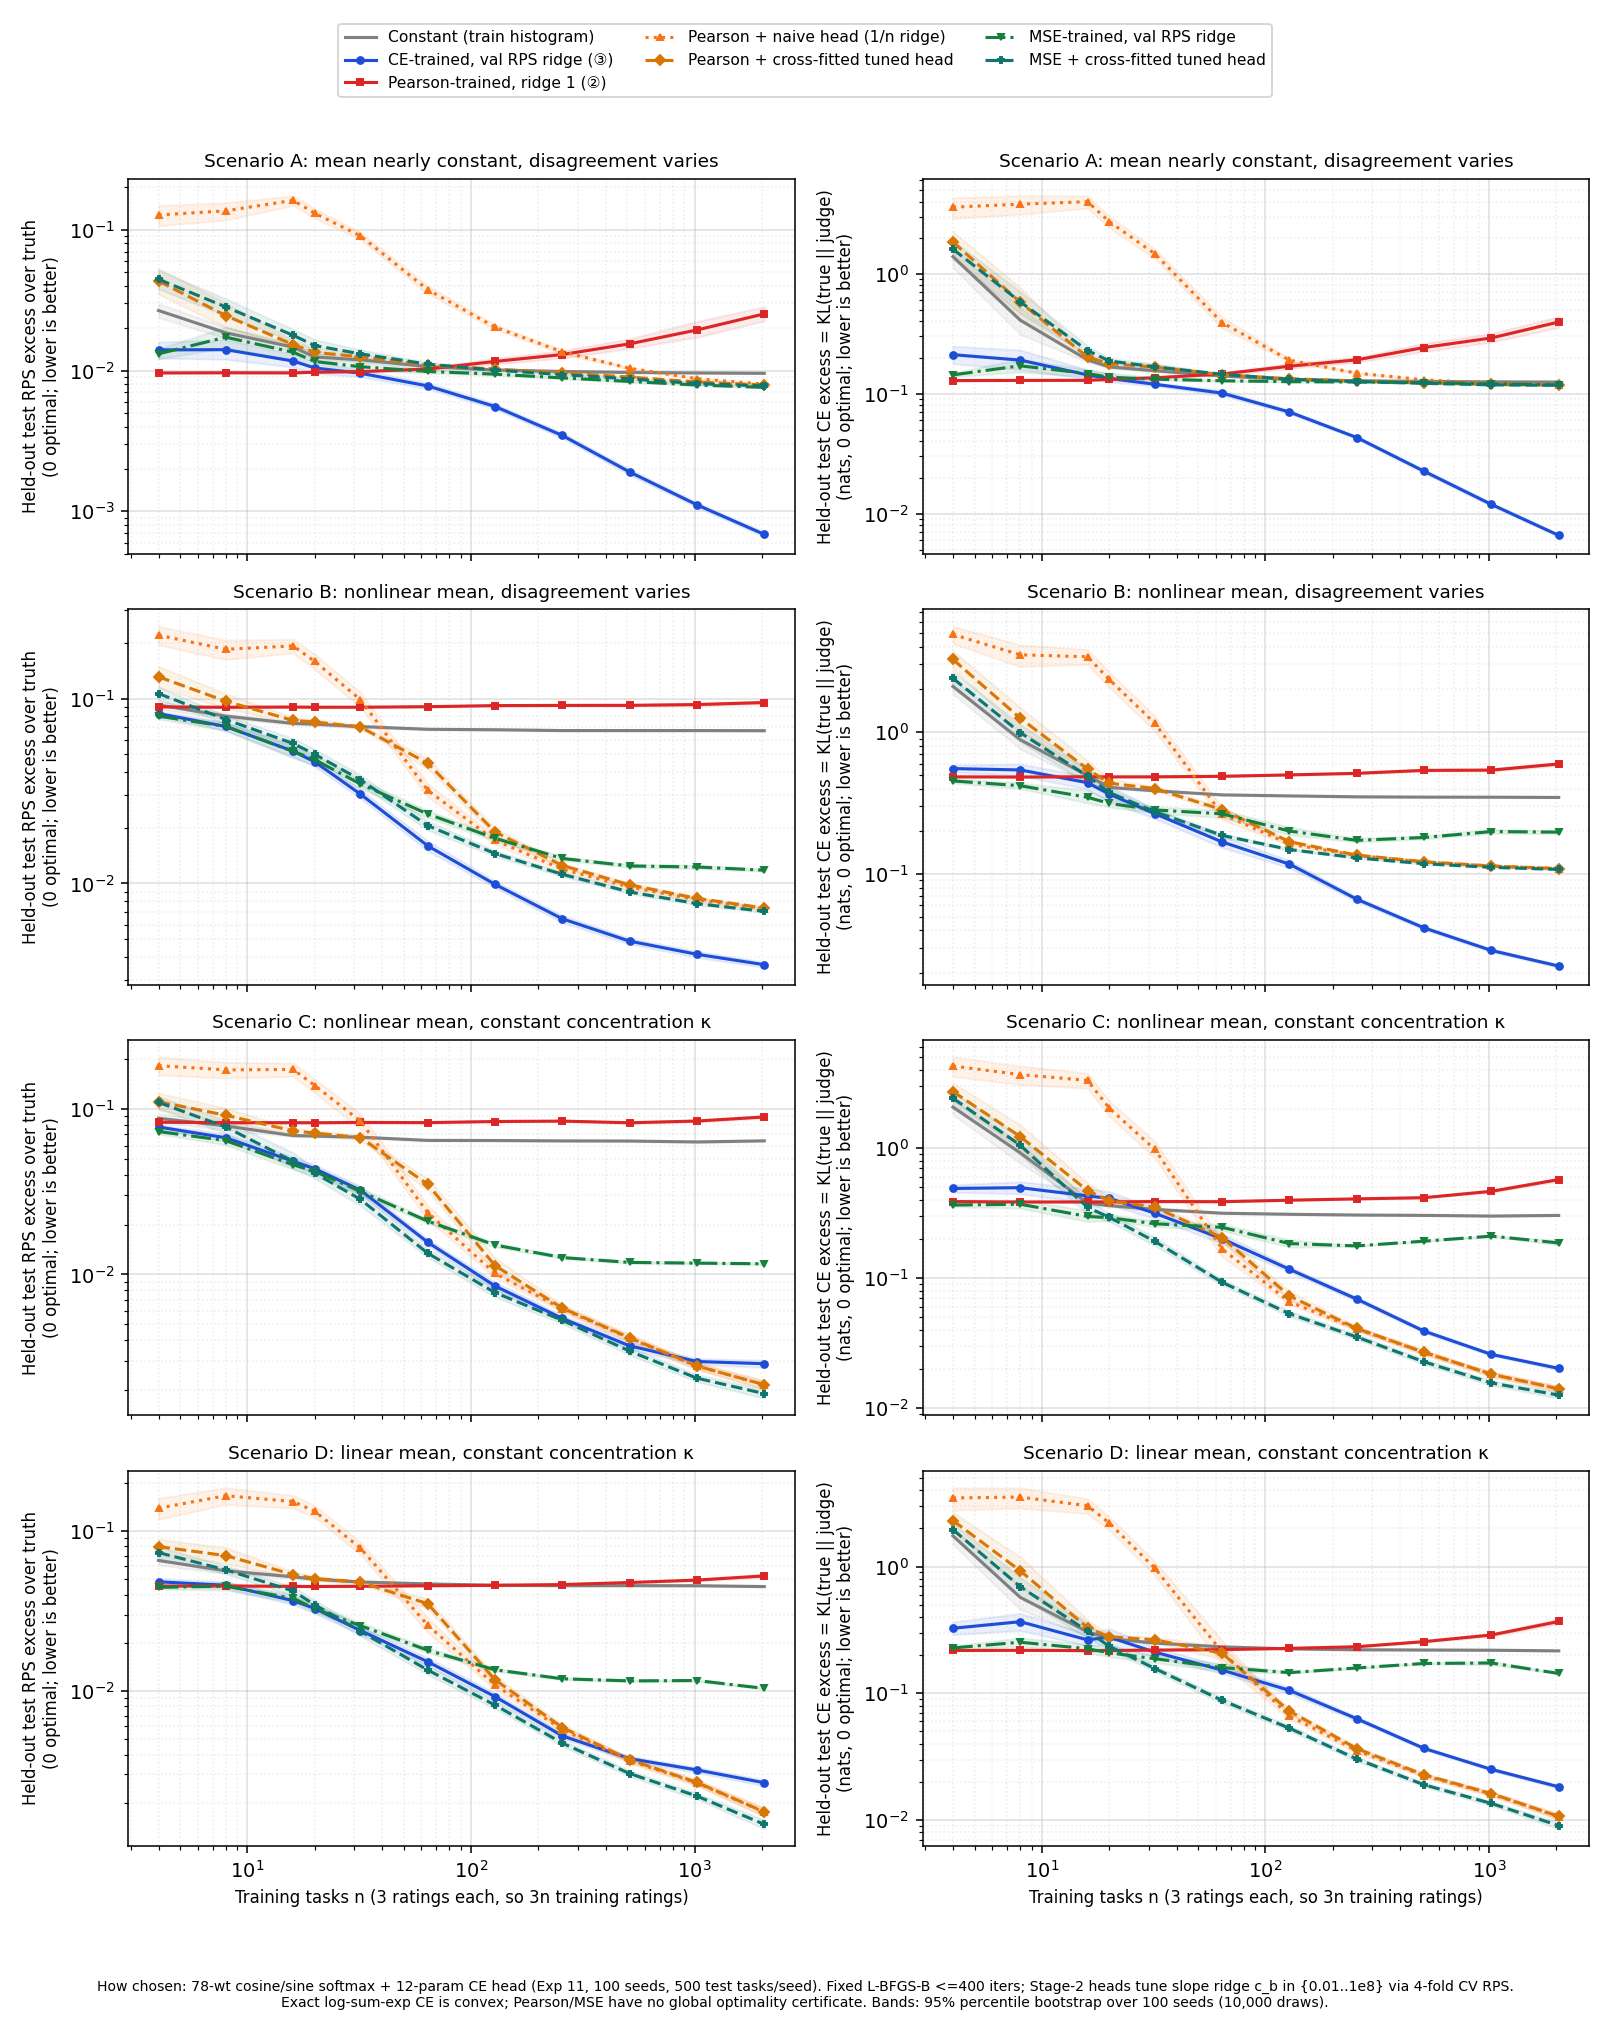
\includegraphics[width=\columnwidth]{figures/fig_mse_and_tuned_head_vs_n.png}
\caption{Experiment~11 held-out test RPS excess (left) and CE excess (right) across Scenarios~A--D comparing exact CE (\textcircled{3}), naive and cross-fitted slope-tuned calibrated heads, and direct 78-weight MSE judges (100 seeds, 500 test tasks/seed; 0 optimal, lower is better).}
\label{fig:supp-exp11}
\end{figure}

\begin{table*}[t]
\centering
\caption{Experiment~11 held-out test RPS excess over truth (and raw RPS vs.\ constant at $n=2{,}048$; 100 seeds, 500 test tasks/seed; 0 optimal, lower is better; paired difference vs.\ \textcircled{3} Val-CE positive means Val-CE is better).}
\label{tab:supp-exp11}
\footnotesize
\setlength{\tabcolsep}{3.5pt}
\begin{tabular}{@{}lccccccc@{}}
\hline
Scenario & Size $n$ & Constant & \textcircled{3} Val-CE & Pearson+Naive & Pearson+Tuned & MSE Val-RPS & MSE+Tuned \\
\hline
A (true $0.187$) & $8$ / $32$ & $0.0185$ / $0.0119$ & $0.0141$ / $0.0096$ & $0.1362$ / $0.0904$ & $0.0245$ / $0.0125$ & $0.0172$ / $0.0106$ & $0.0283$ / $0.0131$ \\
A (raw / ex) & $2{,}048$ & $0.1965$ ($0.0096$) & $0.1876$ ($0.0007$) & $0.1949$ ($0.0080$) & $0.1948$ ($0.0079$) & $0.1945$ ($0.0076$) & $0.1947$ ($0.0078$) \\
B (true $0.136$) & $8$ / $32$ & $0.0803$ / $0.0705$ & $0.0706$ / $0.0304$ & $0.1844$ / $0.0986$ & $0.0967$ / $0.0702$ & $0.0706$ / $0.0345$ & $0.0770$ / $0.0364$ \\
B (raw / ex) & $2{,}048$ & $0.2033$ ($0.0670$) & $0.1400$ ($0.0036$) & $0.1436$ ($0.0073$) & $0.1437$ ($0.0074$) & $0.1481$ ($0.0118$) & $0.1434$ ($0.0071$) \\
C (true $0.127$) & $8$ / $32$ & $0.0788$ / $0.0674$ & $0.0669$ / $0.0322$ & $0.1717$ / $0.0843$ & $0.0914$ / $0.0670$ & $0.0642$ / $0.0317$ & $0.0776$ / $0.0284$ \\
C (raw / ex) & $2{,}048$ & $0.1910$ ($0.0640$) & $0.1299$ ($0.0029$) & $0.1292$ ($0.0022$) & $0.1292$ ($0.0022$) & $0.1386$ ($0.0116$) & $0.1289$ ($0.0019$) \\
D (true $0.146$) & $8$ / $32$ & $0.0563$ / $0.0480$ & $0.0458$ / $0.0238$ & $0.1661$ / $0.0781$ & $0.0701$ / $0.0478$ & $0.0451$ / $0.0256$ & $0.0571$ / $0.0236$ \\
D (raw / ex) & $2{,}048$ & $0.1914$ ($0.0449$) & $0.1492$ ($0.0027$) & $0.1483$ ($0.0017$) & $0.1483$ ($0.0018$) & $0.1569$ ($0.0104$) & $0.1480$ ($0.0015$) \\
\hline
\multicolumn{8}{@{}p{0.94\textwidth}@{}}{At $n=2{,}048$, Pearson+Tuned minus Val-CE [95\% CI]: A $+0.0072$ $[+0.0071,+0.0073]$, B $+0.0037$ $[+0.0036,+0.0038]$, C $-0.0007$ $[-0.0008,-0.0006]$, D $-0.0009$ $[-0.0010,-0.0008]$. MSE Val-RPS minus Val-CE: $+0.0069$ to $+0.0087$ (all CIs $> 0$).} \\
\hline
\end{tabular}
\end{table*}

\section{Extended Open-Weight Breakdown}
\label{sec:supp-open}

All real-judge studies in Experiment~09 evaluate 200 family-disjoint splits ($15$ training task families / $4$ held-out families) from the 75-artifact Python-task rating corpus.
Table~\ref{tab:supp-lora} presents the full numerical LoRA breakdown for the anonymized 4B instruction model and 7B coder model.
In the 48-configuration open-weight family-size learning curve comparing proper-loss training against Pearson across $3$, $9$, and $15$ training families, test RPS improves monotonically from $0.1688$ vs.\ $0.1761$ ($+0.0073$) at 3 families, to $0.1542$ vs.\ $0.1764$ ($+0.0221$ $[+0.0040, +0.0443]$) at 9 families, and to $0.1335$ vs.\ $0.1761$ ($+0.0426$ $[+0.0105, +0.0822]$) at 15 families.

\begin{table*}[t]
\centering
\caption{Experiment~09 open-weight LoRA weight training on anonymized 4B instruction and 7B coder backbones (held-out RPS, CE in nats, signed bias, and MSE; lower is better for RPS, CE, $|\mathrm{bias}|$, MSE).}
\label{tab:supp-lora}
\small
\begin{tabular}{@{}lcccc@{}}
\hline
Judge Variant & Held-Out Test RPS & Held-Out CE (nats) & Signed Bias & MSE \\
\hline
4B Zero-Shot Base & $0.4683$ & --- & --- & --- \\
4B LoRA Pearson & $0.3351$ & --- & $+1.53$ & $4.31$ \\
4B LoRA Spearman & $0.2752$ & --- & --- & --- \\
4B LoRA CE (train / val) & $0.2007$ / $0.1997$ & --- & --- & --- \\
4B LoRA RPS (train) & $0.1887$ & --- & --- & --- \\
4B Pearson-LoRA + 12-param CE Head & $0.1412$ & $1.593$ & --- & --- \\
\hline
7B Zero-Shot Base & $0.4067$ & --- & --- & --- \\
7B LoRA Pearson & $0.4015$ & --- & $+2.11$ & $6.43$ \\
7B LoRA CE (train / val) & $0.1927$ / $0.1859$ & --- & --- & --- \\
7B LoRA RPS (train) & $0.1821$ & --- & --- & --- \\
7B Pearson-LoRA + 12-param CE Head & $0.1560$ & $1.709$ & --- & --- \\
\hline
\end{tabular}
\end{table*}

\section{Frontier Judge Pools and Blind Prompt/Harness Search}
\label{sec:supp-frontier}

Experiment~10 evaluates frontier commercial judge pools in repeated $5\times 5$ family cross-validation, a 250-split 48-configuration sample-size sweep, and a blind $9/5/5$ split (30 held-out test artifacts) optimizing discrete prompt wording and harness wrappers.
Table~\ref{tab:supp-frontier-pools} lists all pool results (\texttt{Hist-5} historical three-call configurations, \texttt{Native-15} native six-probability configurations, and \texttt{Combined-20}).
Figure~\ref{fig:supp-frontier-curve} traces the 48-configuration frontier family-count curve across $250$ splits: at $3$ families, mean RPS values for (\textcircled{4} CE, \textcircled{3} Val-CE, \textcircled{2} Pearson, Pearson+Head) are $(0.1848, 0.1883, 0.1814, 0.2303)$; at $9$ families, $(0.1771, 0.1735, 0.1815, 0.1873)$; and at $15$ families, $(0.1569, 0.1290, 0.1819, 0.1301)$.
Finally, Table~\ref{tab:supp-frontier-live} reports the blind live prompt-and-harness search over the $9/5/5$ task-family split ($30$ test artifacts).
Under the basic prompt/harness \texttt{H1}, validation-Pearson selection ($0.1828$) trails training-Pearson selection ($0.1068$), while CE selection reaches $0.1410$ despite $7/30$ items reverting to uniform fallback probability predictions under structured formatting checks.
Under the richer structured harness \texttt{H3}, base $0.1600$ improves to $0.1136$ under \texttt{P\_corr\_val} and $0.1174$ under \texttt{P\_ce\_val}.
When choosing jointly over prompts and harnesses on validation, the difference between RPS-selected and Pearson-selected judges is $-0.0060$ ($95\%$ CI $[-0.0493, +0.0613]$; $0.1529$ vs.\ $0.1590$), remaining statistically indistinguishable at this 5-family validation budget.

\begin{figure}[t]
\centering
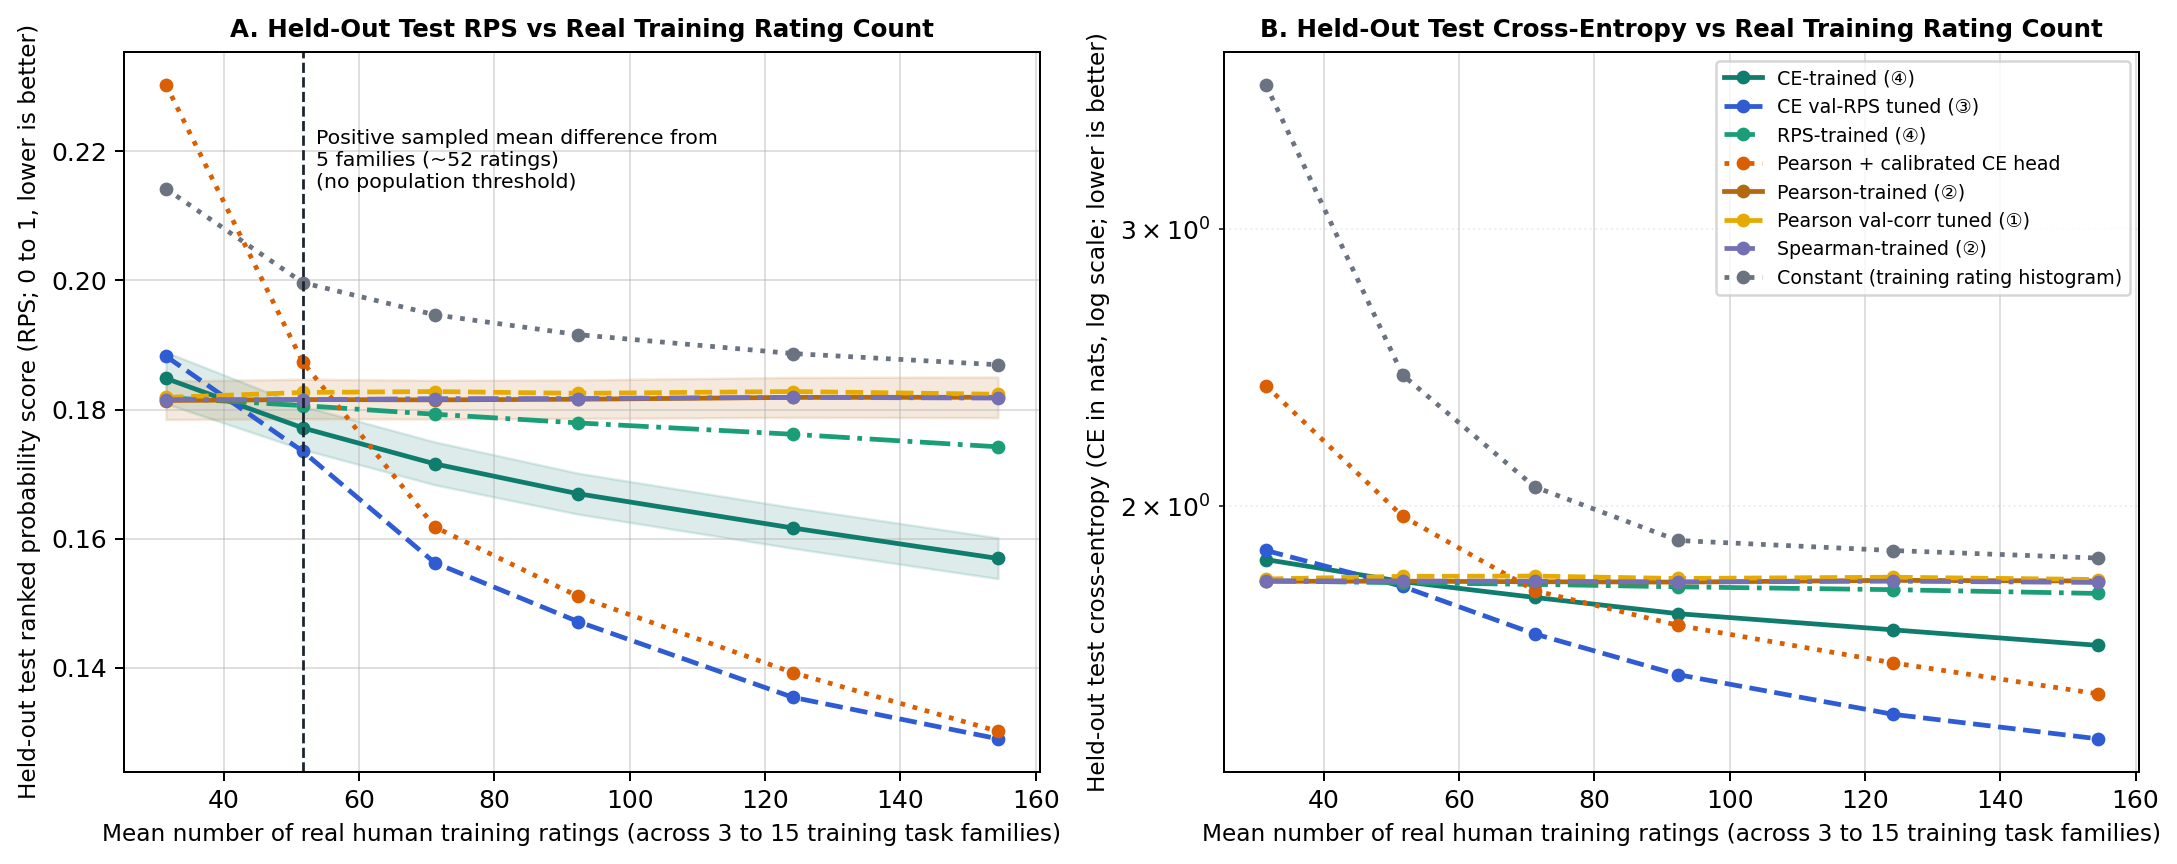
\includegraphics[width=\columnwidth]{figures/fig3_learning_curve_vs_ratings.png}
\caption{Experiment~10 frontier 48-configuration held-out test RPS versus number of training task families ($3$, $9$, and $15$ families over $250$ family-disjoint splits) comparing Formulations~\textcircled{4} CE-train, \textcircled{3} Val-CE, \textcircled{2} Pearson-train, and Pearson + calibrated head.}
\label{fig:supp-frontier-curve}
\end{figure}

\begin{table*}[t]
\centering
\caption{Experiment~10 frontier pool evaluation across \texttt{Hist-5}, \texttt{Native-15}, and \texttt{Combined-20} ($5\times 5$ repeated family CV; lower is better).}
\label{tab:supp-frontier-pools}
\small
\begin{tabular}{@{}lcc@{}}
\hline
Pool & Selection / Training Method & Held-Out Test RPS (CE nats) \\
\hline
\texttt{Hist-5} & Constant baseline & $0.1872$ ($1.928$) \\
\texttt{Hist-5} & Equal-weight mix & $0.1496$ ($5.431$) \\
\texttt{Hist-5} & \textcircled{4} CE-mix / RPS-mix / Pearson-mix & $0.1391$ ($5.491$) / $0.1350$ ($5.757$) / $0.1436$ ($5.752$) \\
\texttt{Hist-5} & Single (CE / RPS / Pearson) & $0.2032$ / $0.2154$ / $0.1793$ \\
\hline
\texttt{Native-15} & \textcircled{4} CE-mix / \textcircled{3} Val-CE / RPS-mix & $0.1137$ ($1.416$) / $0.1136$ ($1.416$) / $0.1166$ ($1.445$) \\
\texttt{Native-15} & \textcircled{2} Pearson-mix (bias $+1.129$) & $0.1912$ ($1.971$) \\
\texttt{Native-15} & Single (CE / RPS / Pearson) & $0.1252$ / $0.1360$ / $0.1426$ \\
\hline
\texttt{Combined-20} & \textcircled{4} CE-mix / \textcircled{3} Val-CE / RPS-mix & $0.1092$ ($1.389$) / $0.1091$ ($1.389$) / $0.1093$ ($1.437$) \\
\texttt{Combined-20} & \textcircled{2} Pearson-mix / Single Pearson & $0.1671$ / $0.1848$ \\
\hline
\end{tabular}
\end{table*}

\begin{table*}[t]
\centering
\caption{Experiment~10 blind frontier prompt and harness search on the held-out $9/5/5$ split (30 test items; lower RPS is better).}
\label{tab:supp-frontier-live}
\small
\begin{tabular}{@{}llc@{}}
\hline
Harness & Prompt Variant & Held-Out Test RPS \\
\hline
\texttt{H1} (basic) & Baseline \texttt{P0\_H1} & $0.1812$ \\
\texttt{H1} (basic) & Validation-Pearson \texttt{P\_corr\_val} & $0.1828$ \\
\texttt{H1} (basic) & Train-Pearson \texttt{P\_corr\_tr} & $0.1068$ \\
\texttt{H1} (basic) & Validation-CE \texttt{P\_ce\_val} ($7/30$ fallbacks) & $0.1410$ \\
\hline
\texttt{H3} (structured) & Baseline \texttt{P0} & $0.1600$ \\
\texttt{H3} (structured) & Validation-Pearson \texttt{P\_corr\_val} & $0.1136$ \\
\texttt{H3} (structured) & Validation-CE \texttt{P\_ce\_val} & $0.1174$ \\
\hline
Joint $2\times 2$ Val & RPS-selected vs.\ Pearson-selected & $0.1529$ vs.\ $0.1590$ ($-0.0060$ $[-0.0493,+0.0613]$) \\
\hline
\end{tabular}
\end{table*}

\section{Data Provenance, Validity Limitations, and Optimization Scope}
\label{sec:supp-validity}

Four empirical boundaries govern interpretation of the human-rating and synthetic studies:
\begin{enumerate}
    \item \emph{Retrospective sample reuse and artifact reference mismatch.} All real-judge experiments share one retrospective 75-artifact pool (25 tasks, 19 families).
    Furthermore, only $15/75$ on-disk reference hashes match annotation metadata ($60/75$ differ), leaving exact byte provenance of historical delivered references unverified outside prospective collection.
    \item \emph{Prior dataset exposure.} In the frontier model tests, some baseline configurations reflect prompts inspected earlier on overlapping tasks, motivating the separate blind $9/5/5$ split where validation and test prompts remained strictly unseen during search.
    \item \emph{Rater count vs.\ severity.} Because each retrospective artifact receives only $2$--$3$ human ratings, constant rater offsets are estimable and small (about $0.1$ rating points, about $2\%$ of within-artifact variance), but rater-by-item interaction and rater use of the scale cannot be disentangled from inherent item ambiguity.
    Where rating variance stems predominantly from rater noise rather than genuine item disagreement, predicting the expected universe score becomes the appropriate target rather than reproducing noisy per-rater dispersion.
    \item \emph{Optimizer budget on nonconvex objectives.} Synthetic results reflect finite-budget L-BFGS-B optimization ($400$--$2{,}000$ iterations across $1$--$9$ starts).
    While convex CE guarantees unique optima verified across $95{,}291$ exact-gradient refits, rank and correlation objectives lack global optimality certificates, strengthening the practical recommendation to prefer convex proper losses whenever flexible parameters are trained.
\end{enumerate}
